\section{Visualisation}
%what are the features we want to emphasis?
%make a bullet list of something like that
Our goal is to design an interactive visualisation system on top of the structured prediction framework.
Figure~\ref{fig:overview} shows the overview of a live demo system, which consists of four major components: a map to display suggested routes, an input box for user query (upper left), a stacked score of routes (upper right), and a radar chart to compare multiple POIs (lower right). 
The role and the construction of three major components, besides the main map, are as follows:

%\begin{itemize}
\textbf{Query input}: A query consists of a starting POI and a trip length. 
Users can choose the starting POI by clicking icons on the map and can adjust the slide to set the trip length. 
In addition, three different travelling modes (e.g. bicycling, walking, and driving) are supported, 
and we optimise the suggested routes for each mode.

\textbf{Route score visualisation}: Ranks of candidate routes are determined by their total scores from the SSVM. 
The score of each route can be decomposed into scores for each POI and edge along the route. 
We adopt the LineUp framework~\cite{gratzl2013lineup} designed to support the visualisation of multi-attribute ranking via stacked representation. 
Figure~\ref{fig:stack} shows the stacked representation of the top ten scored routes, where the proportion of each bar indicates the importance of each POI in the route.

\textbf{POI feature visualisation}: We further provide a tool to analyse the variation between POIs in a single route. 
        For example, in Figure~\ref{fig:radar}, we compare two POIs, the \textit{Queen Victoria Market} and \textit{Melbourne Aquarium}, in terms of POI features and their importance in the suggested route. 
%\end{itemize}

\begin{figure}[t!]
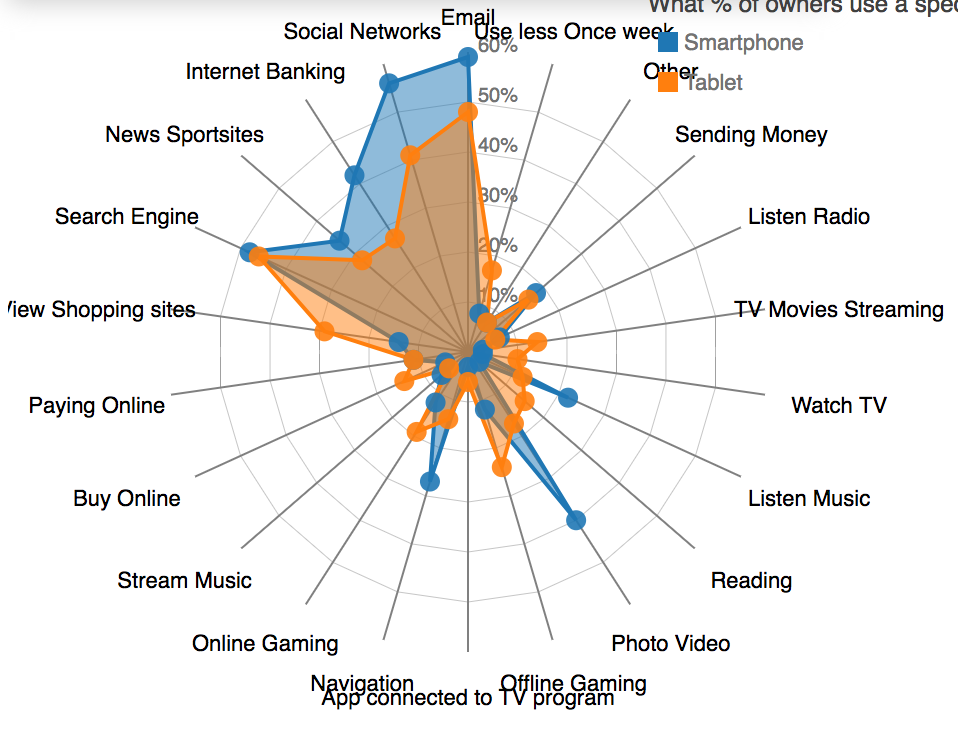
\includegraphics[width=0.6\linewidth]{figure/sample_radar.png}
    \caption{POI feature comparison between \textit{Melbourne Aquarium} and \textit{Queen Victoria Market}: the former scores higher on \textit{Popularity} and \textit{Visits difference} features whereas the latter scores higher on \textit{Visits} and \textit{Popularity difference} features.}
\label{fig:radar} \vspace{-1em}
\end{figure}
